\chapter{Tree}


\section{Binary Search Tree}
The search binary tree data structure is capable of suporting both \textit{dictionary} and \textit{priority queue} operation in time proportional to the height of the tree.
Note that in the average case, for randomly constructed tree , the hight is $\Theta(log n)$ but the worst case is bad, since there is always a way to arrange it items s.t. it degrade to a linked list, with height $O(n)$. Self balancing trees ensure that the hight is always logaritmic in the number of nodes (red-black, or AVL tree are two names for such trees).

Let's start stating what is the invariant that makes the binary search tree so powerful. The binary search property always hold for each node of the tree, and all the operations always manintain such property.


\textbf{For each node of the three $x$ then all the nodes in the left subtree rooted at $x.left$ are strictly smaller  then $x.key$ and all the nodes in the right subtree rooted at $x.right$ are greater or equal than $x.key$.
}

	\begin{figure}
	\label{fig:tree_visits}
	\centering
		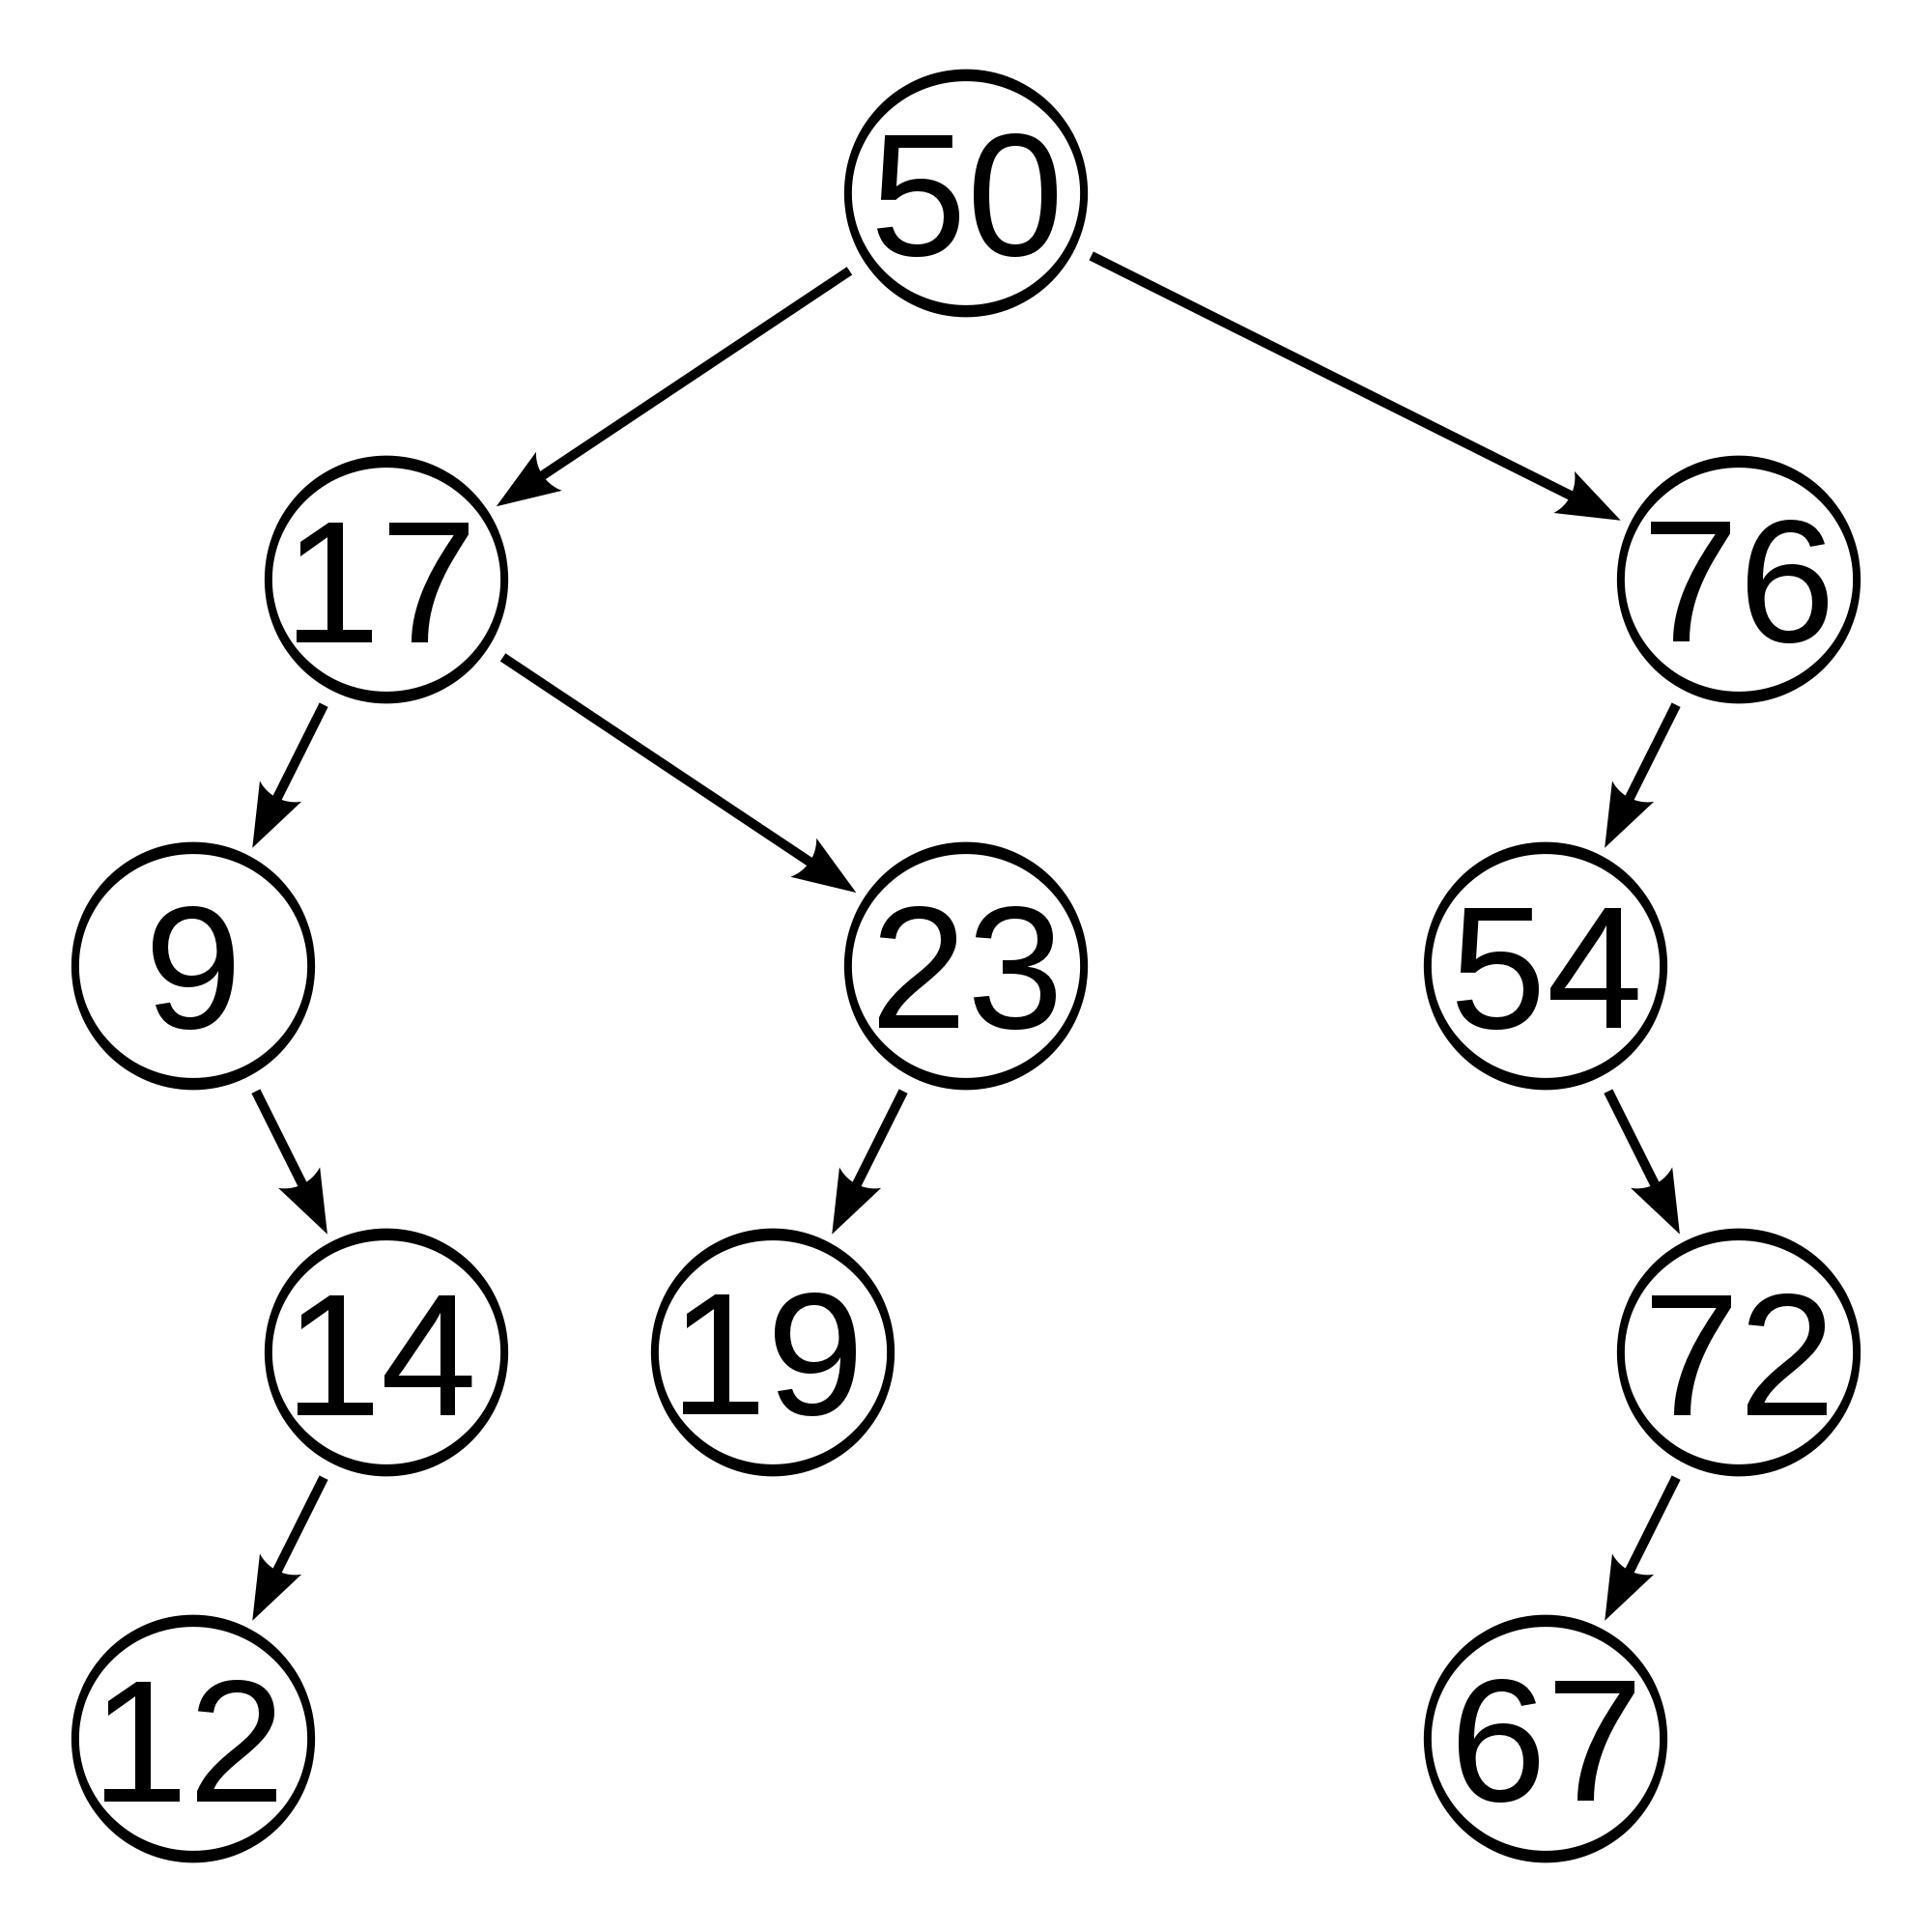
\includegraphics[scale=0.1]{../images/tree_unbl}
		\caption{Binary search tree}
	\end{figure}

It's important to notice the difference between the binary search property and the heap property. The heap property states that for each nodes, the key of the children  of a node $x$ have to be lesser the $x.key$ (both of them). The minimum element is then the root of the tree. Min heap property is less string, and hence easier to mantain, but makes the heap less poweful than the binary search tree. For instance search in a heap costs linear time. Moreover the heap is not able to print out all the element it stores in \textbf{sorted order} in linear time. It takes $\Theta(nlogn)$ since at each min extraction the min heap needs to be restored bubbling up some nodes from the new root to the leaf (in $O(log n)$) 

It is possible to print all the element stored in a search tree in sorted order simply using the so called \textbf{in order} visit of the tree. Given a tree rooted at $x$ is first visit all the nodes of the left subtree, then prints the key of $x$, and finally prints all the nodes in the right subtree.



\begin{algorithm}
\Fn{IN-ORDER(x)}{
		\If{$x=NIL$}{
			\Return \;		
		}	
		$IN-ORDER(x.left)$\;
		$process(x.key)$\;
		$IN-ORDER(x.right)$\;
	}
\caption{In order visi of a binary (search) tree }
\end{algorithm}

Intuitively this works because  the recursion walk down the leftmost path of the tree first reaching the minimum element (which is always a leaf) then prints the that element and recurs on its right subtree if present. Again starting from this node we walk our way down to the leftmost subtree, which in other word is the smallest element among all the greater element of the element just printed out. This is the successor of the printed element! So we alway print an element and its successor.

Changing the order in which we process the node and the recursive calls will make us visit the tree in different order. There are other two ways to arrange the recursive calls and the process the node (see algorithms \ref{alg:pre} and \ref{alg:pst}). 
\begin{itemize}
\item the \textbf{pre-order} visit process the current node first and then recursively visit the left and right subtrees.
\item the \textbf{post-order} visit, as the name suggest processs the current node after processing left and right subtree.
\end{itemize}


\begin{algorithm}
\Fn{PRE-ORDER(x)}{
		\If{$x=NIL$}{
			\Return \;		
		}	
		$process(x.key)$\;
		$IN-ORDER(x.left)$\;
		$IN-ORDER(x.right)$\;
	}
\caption{Pre order visi of a binary (search) tree }\label{alg:pre}
\end{algorithm}


\begin{algorithm}
\Fn{POST-ORDER(x)}{
		\If{$x=NIL$}{
			\Return \;		
		}	
		
		$IN-ORDER(x.left)$\;
		$IN-ORDER(x.right)$\;
		$process(x.key)$\;
	}
\caption{Post order visi of a binary (search) tree }\label{alg:pst}
\end{algorithm}

What is the running time of a such visit on a tree composed of $n$ nodes?
We should start noticing that a visit at least print all the elements once so its running time canno be less than $\Omega(n)$.
Noticing that no nodes is accessed twice gives us that the running time is also $O(n)$. This allows us to conclude that the running time is in reality $\Theta(n)$.

It is important to notice that the visit can also be implemented in a non-recursive procedure. non-recursive calls can be important when the height of the tree is not garanteed to be logaritmic in the number of nodes. Infact when logaritmic the recursive stack of calls has logaritmic length which is not a problem even on tree of a million elements. If the tree ha linear height, on the other hand, this could cause a stack error.

FThe in order walk can be implemented using a stack as an auxiliary data structure that stores the nodes to be processed (taking care of not adding any $NIL$) and whenever we traverse on a $NIL$ subtree we pop from the stack (which contains a valid element), process that element and go right.

\begin{algorithm}
\Fn{IN-ORDER-ITERATIVE(x,S)}{
		$S.push(x)$\;
		$current=x$\;
		\While{$S.size() > 0$}{
			\eIf{$current \neq NIL$}{
			\If{$current.left\neq NIL$}{
					$S.push(current.left)$\;
					
				}
			$current=current.left$
			}{
				$current=S.pop()$\;
				$process(p)$\;
				\If{$current.right \neq NIL$}{
				$S.push(current.right)$\;
				}
				$current=current.right$
			}
		}
		
	}
\caption{In order iterative visit }\label{alg:pst}
\end{algorithm}

The pre-order iterative visit can be implemented using a queue instead of a stack. The root is enqueued and while the queue is not empty we extract an element from the queue and process it straight away. Then we add, if present, left (first) and right children.

\begin{algorithm}
\Fn{PRE-ORDER-ITERATIVE(x,Q)}{
		$Q.push(x)$\;
		\While{$S.size() > 0$}{
			$current=Q.dequeue()$\;
			$process(p)$\;
			\If{$current.left\neq NIL$}{
				$Q.enqueue(current.left)$\;
			}
			\If{$current.right \neq NIL$}{
				$S.push(current.right)$\;
				}
	
			}
		}
\caption{Pre order iterative visit }\label{alg:pre_iter}
\end{algorithm}




\section{Self Balancing Tree}
\subsection{B Tree}
\subsection{B+ Tree}

\subsection{Adelson-Velsky Landis Tree - AVL Tree}
\subsection{Red Black Tree}
\subsection{Splay Tree}


\section{Space-partitioning trees}
\subsection{Kd Tree}
\subsection{R Tree}